% Options for packages loaded elsewhere
\PassOptionsToPackage{unicode}{hyperref}
\PassOptionsToPackage{hyphens}{url}
%
\documentclass[
]{article}
\usepackage{amsmath,amssymb}
\usepackage{lmodern}
\usepackage{iftex}
\ifPDFTeX
  \usepackage[T1]{fontenc}
  \usepackage[utf8]{inputenc}
  \usepackage{textcomp} % provide euro and other symbols
\else % if luatex or xetex
  \usepackage{unicode-math}
  \defaultfontfeatures{Scale=MatchLowercase}
  \defaultfontfeatures[\rmfamily]{Ligatures=TeX,Scale=1}
\fi
% Use upquote if available, for straight quotes in verbatim environments
\IfFileExists{upquote.sty}{\usepackage{upquote}}{}
\IfFileExists{microtype.sty}{% use microtype if available
  \usepackage[]{microtype}
  \UseMicrotypeSet[protrusion]{basicmath} % disable protrusion for tt fonts
}{}
\makeatletter
\@ifundefined{KOMAClassName}{% if non-KOMA class
  \IfFileExists{parskip.sty}{%
    \usepackage{parskip}
  }{% else
    \setlength{\parindent}{0pt}
    \setlength{\parskip}{6pt plus 2pt minus 1pt}}
}{% if KOMA class
  \KOMAoptions{parskip=half}}
\makeatother
\usepackage{xcolor}
\IfFileExists{xurl.sty}{\usepackage{xurl}}{} % add URL line breaks if available
\IfFileExists{bookmark.sty}{\usepackage{bookmark}}{\usepackage{hyperref}}
\hypersetup{
  pdftitle={Model\_Description},
  hidelinks,
  pdfcreator={LaTeX via pandoc}}
\urlstyle{same} % disable monospaced font for URLs
\usepackage[margin=1in]{geometry}
\usepackage{graphicx}
\makeatletter
\def\maxwidth{\ifdim\Gin@nat@width>\linewidth\linewidth\else\Gin@nat@width\fi}
\def\maxheight{\ifdim\Gin@nat@height>\textheight\textheight\else\Gin@nat@height\fi}
\makeatother
% Scale images if necessary, so that they will not overflow the page
% margins by default, and it is still possible to overwrite the defaults
% using explicit options in \includegraphics[width, height, ...]{}
\setkeys{Gin}{width=\maxwidth,height=\maxheight,keepaspectratio}
% Set default figure placement to htbp
\makeatletter
\def\fps@figure{htbp}
\makeatother
\setlength{\emergencystretch}{3em} % prevent overfull lines
\providecommand{\tightlist}{%
  \setlength{\itemsep}{0pt}\setlength{\parskip}{0pt}}
\setcounter{secnumdepth}{-\maxdimen} % remove section numbering
\ifLuaTeX
  \usepackage{selnolig}  % disable illegal ligatures
\fi

\title{Model\_Description}
\author{}
\date{\vspace{-2.5em}2022-05-11}

\begin{document}
\maketitle

\hypertarget{si-characteristics}{%
\section{SI-Characteristics}\label{si-characteristics}}

The following were the initial SI-Characteristics decided through
preliminary research and discussion rounds:

\begin{figure}

{\centering 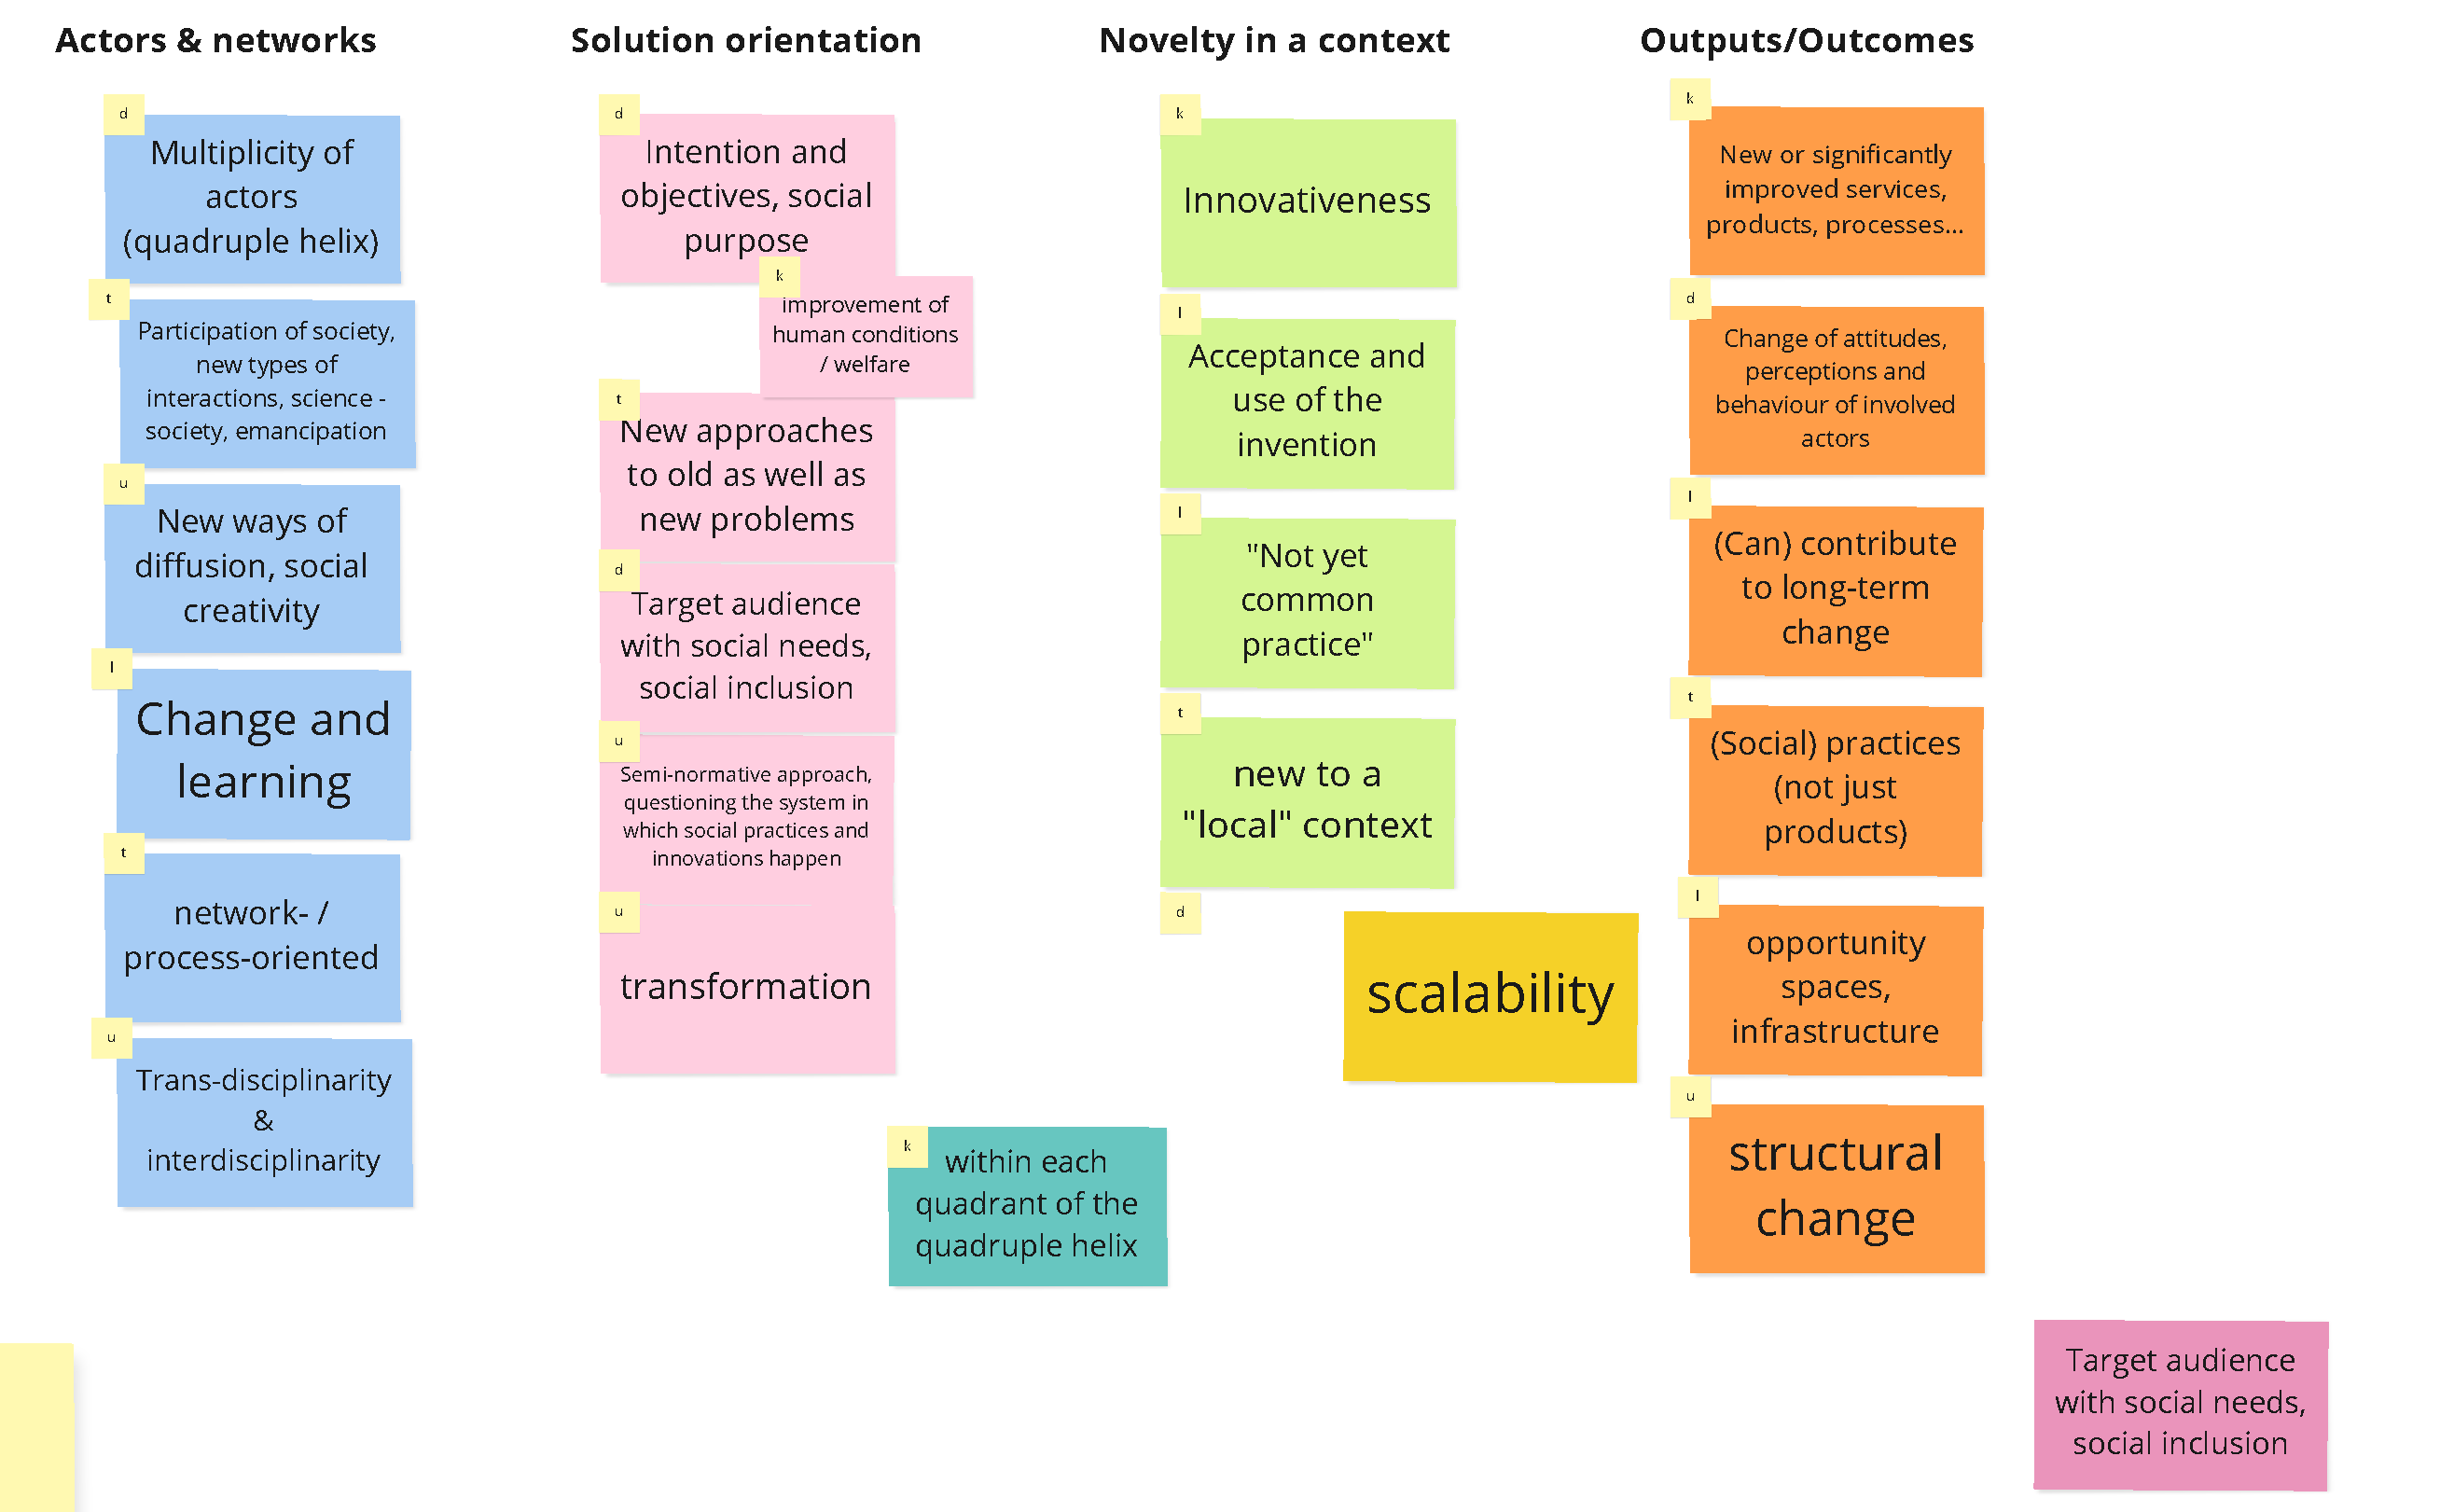
\includegraphics[width=0.3\linewidth]{../06_model/SIVOCS - SI characteristics} 

}

\caption{your caption}\label{fig:unnamed-chunk-2}
\end{figure}

\hypertarget{variable-preprocessing}{%
\section{Variable Preprocessing}\label{variable-preprocessing}}

The elimination of the variables relied on 2 different type of
considerations:

\begin{itemize}
\item
  Elimination by Principal Feature Analysis
\item
  Explained Variance
\end{itemize}

\hypertarget{principal-feature-analysis}{%
\subsection{Principal Feature
Analysis}\label{principal-feature-analysis}}

After the 1000 iterations of PFA, the following are the frequency of
each variable being in the ``significant'' variables list:

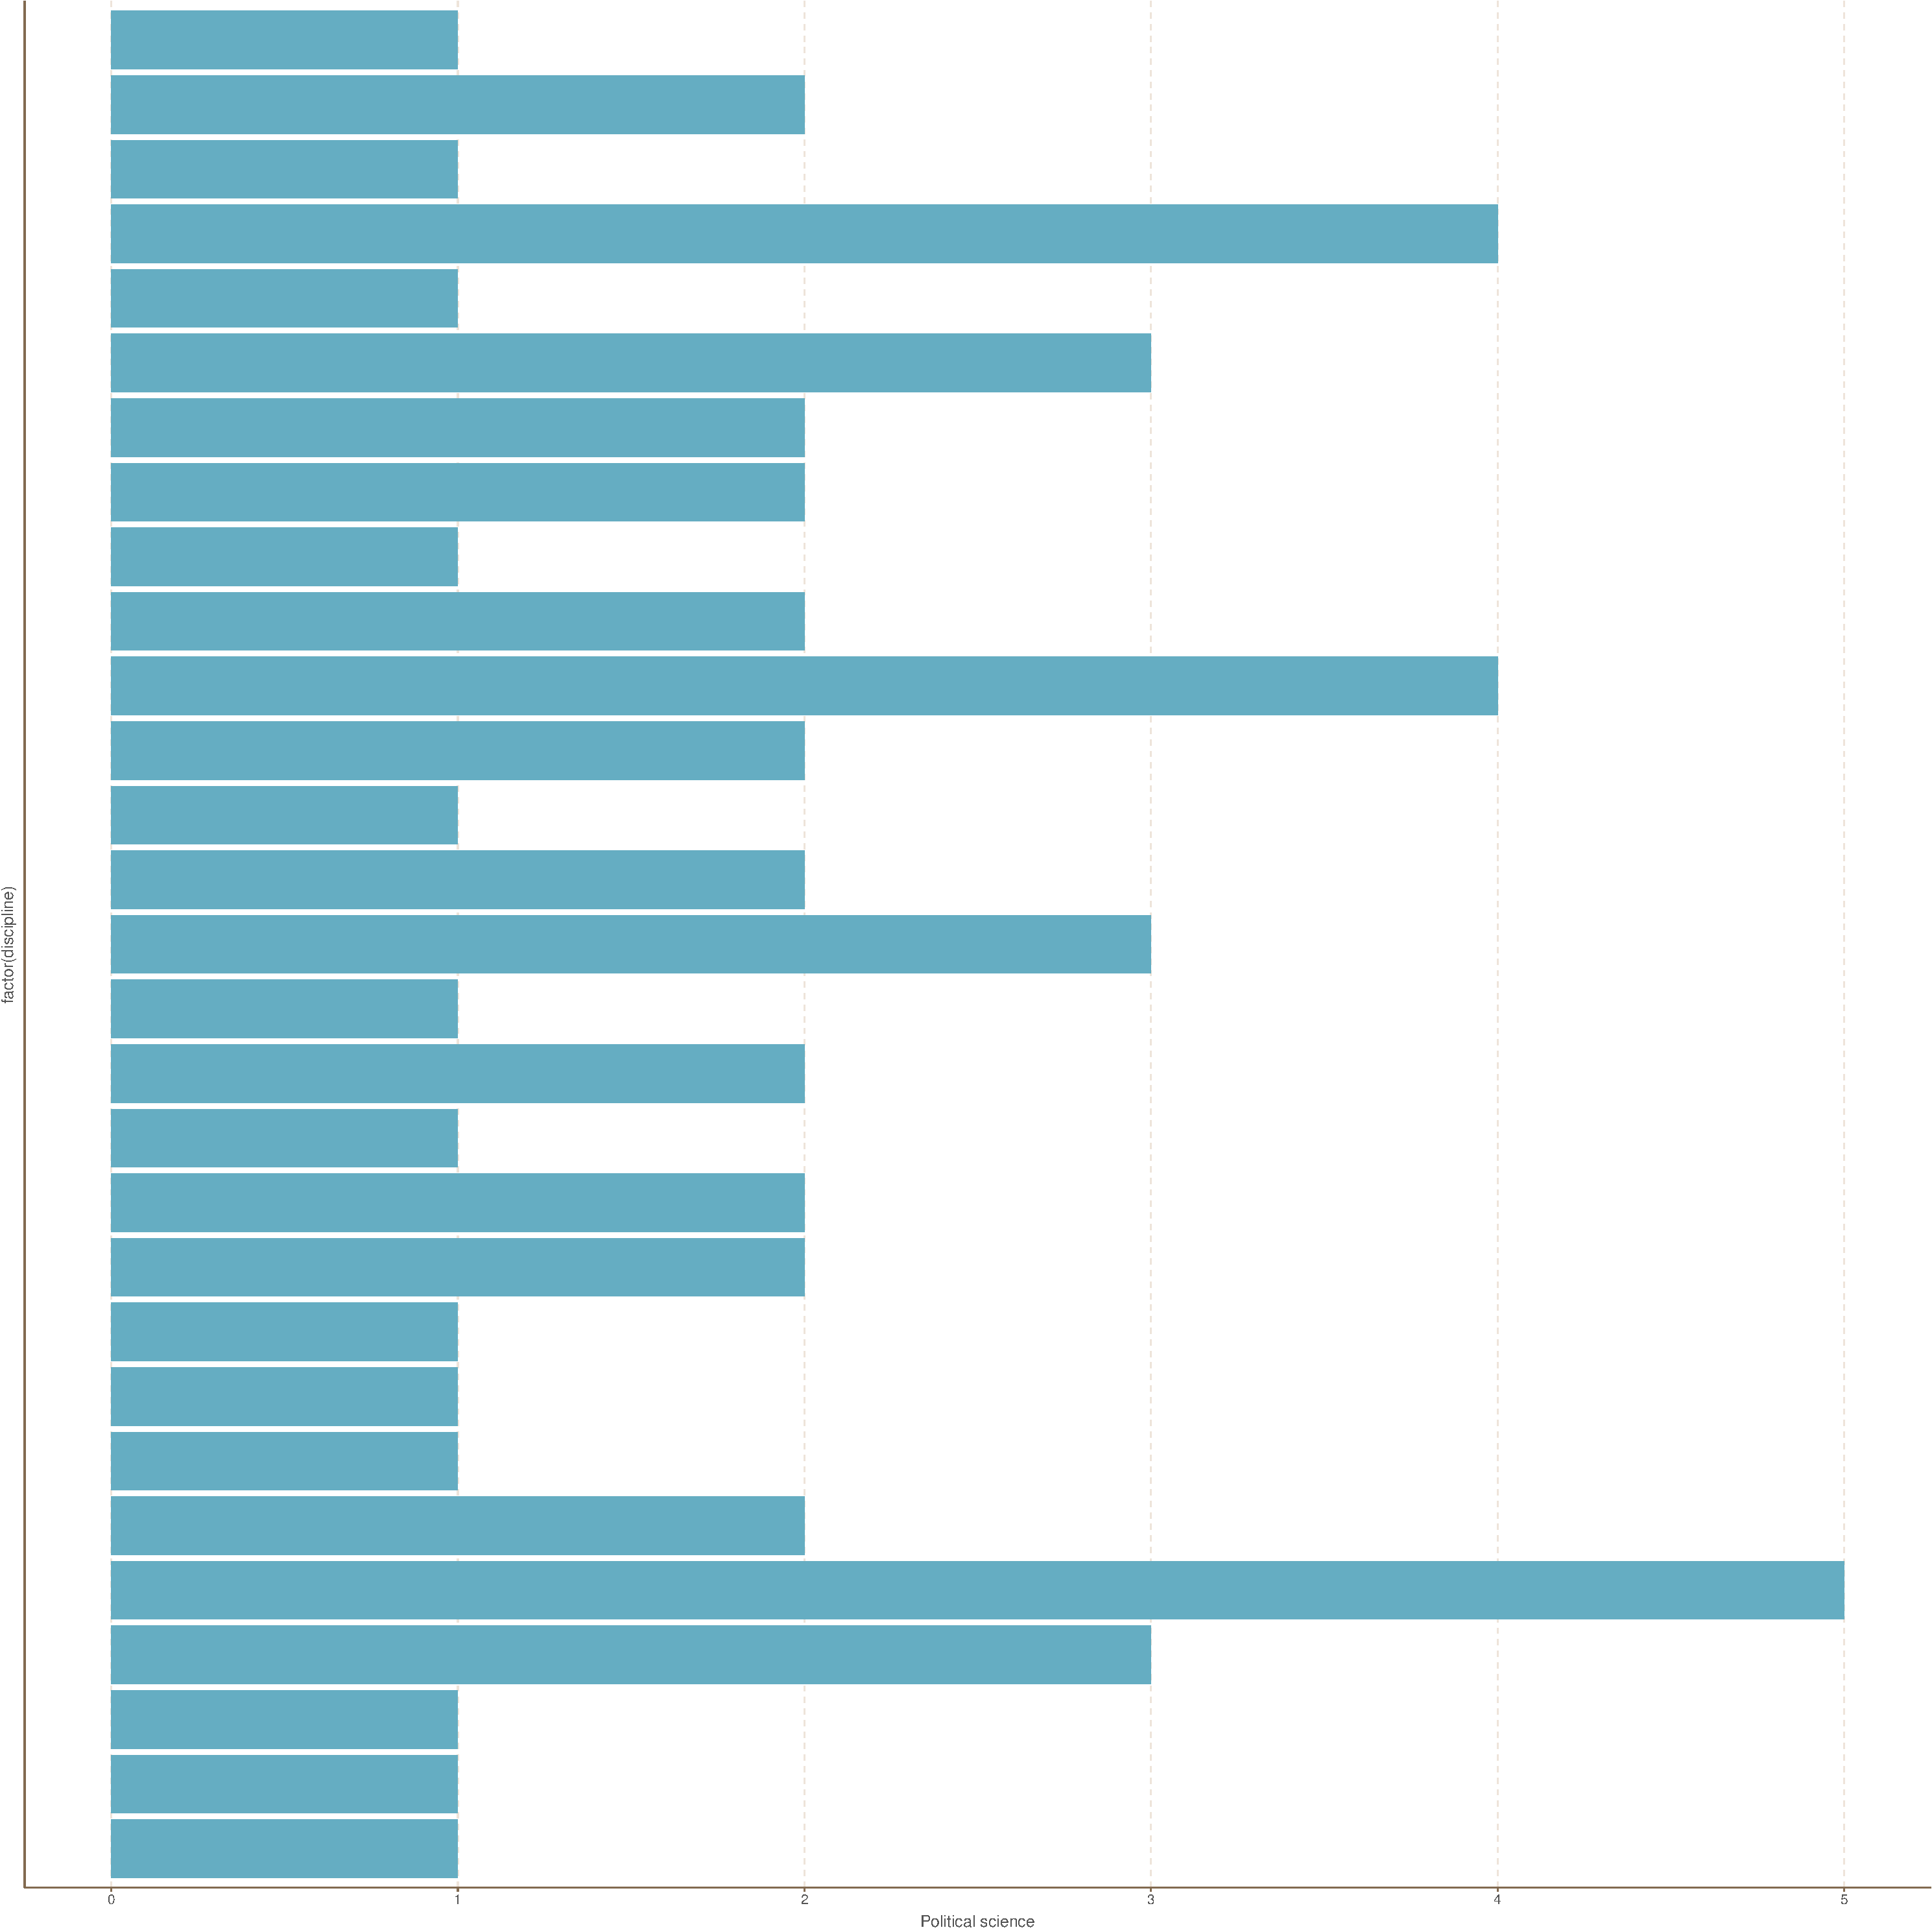
\includegraphics{model_description_files/figure-latex/unnamed-chunk-4-1.pdf}

\hypertarget{removed-features}{%
\subsection{Removed Features}\label{removed-features}}

Note: Some of the features have been kept despite being rated low
importance by PFA

``dissChannels.platf.'' ``dissChannels.prof.''\\
``dissChannels.mono.'' ``concepts.review.''\\
``adoptByPolicyHow.SQ002.'' ``dissChannels.peer.''\\
``dissChannels.policy.'' ``concepts.pub.''\\
``natureOfInvolvement.busi.'' ``dissChannels.web.''\\
``concepts3'' ``dissChannels.conf.''\\
``adoptByPolicy.rate.'' ``adoptByPolicyHow.SQ003.''\\
``dissChannels.trad.'' ``dissChannels.socmed.''\\
``dissChannels.consult.'' ``dissChannels.events.''\\
``dissChannels.public.'' ``concepts.data.''\\
``concepts.code.'' ``concepts.infra.''\\
``contribToSI.rate.'' ``groupsInvolved.res.''\\
``natureOfInvolvement.res.'' ``contribToSI.rate.''

\hypertarget{model-approach-considerations}{%
\section{Model Approach
Considerations}\label{model-approach-considerations}}

\hypertarget{factor-analysis}{%
\subsection{Factor analysis}\label{factor-analysis}}

\hypertarget{scree-plot}{%
\subsubsection{Scree Plot}\label{scree-plot}}

Determine Number of Factors to Extract

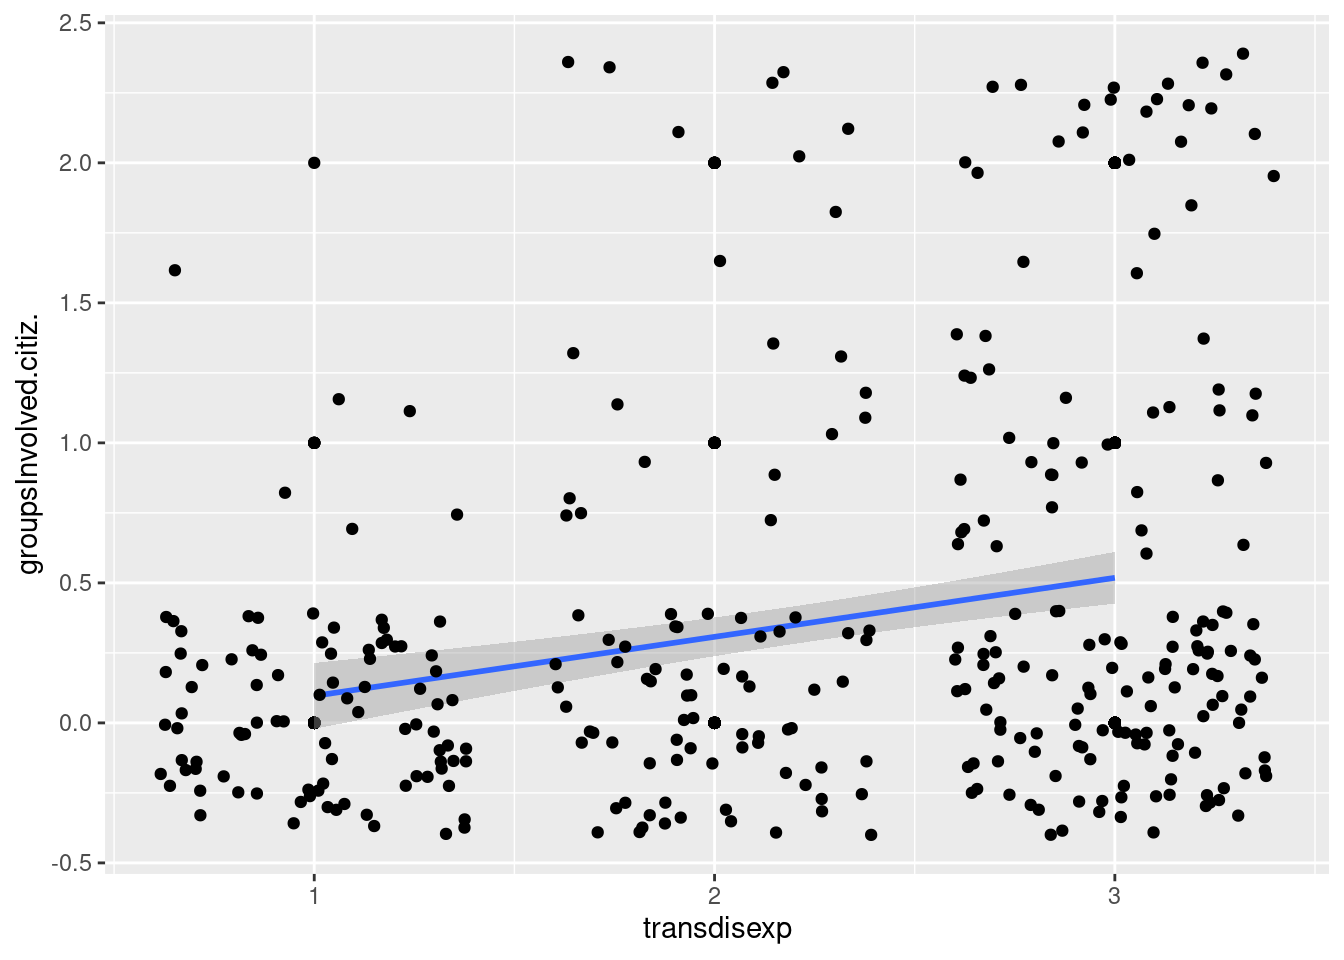
\includegraphics{model_description_files/figure-latex/unnamed-chunk-6-1.pdf}
The optimal number of factors is 8

\hypertarget{exploratory-factor-analysis}{%
\subsection{Exploratory Factor
Analysis}\label{exploratory-factor-analysis}}

\begin{verbatim}
## 
## Call:
## factanal(x = df_red, factors = 8, rotation = "varimax")
## 
## Uniquenesses:
##      transdisciplinaryExp.rate.        familiarWithSI.response. 
##                            0.75                            0.66 
##               motivation.pheno.                motivation.prob. 
##                            0.95                            0.90 
##             motivation.welfare.            benefitForNonAcademy 
##                            0.39                            0.32 
##          impulseForNonAcad.soc.         impulseForNonAcad.econ. 
##                            0.54                            0.77 
##         impulseForNonAcad.ecol.       impulseForNonAcad.health. 
##                            0.83                            0.63 
##         impulseForNonAcad.tech.            groupsInvolved.busi. 
##                            0.92                            0.25 
##          groupsInvolved.civsoc.          groupsInvolved.policy. 
##                            0.20                            0.24 
##           groupsInvolved.citiz.           groupsInvolved.media. 
##                            0.52                            0.76 
##         groupsInvolved.welfare.       natureOfInvolvement.busi. 
##                            0.33                            0.19 
##     natureOfInvolvement.civsoc.     natureOfInvolvement.policy. 
##                            0.37                            0.60 
##      natureOfInvolvement.citiz.      natureOfInvolvement.media. 
##                            0.64                            0.90 
##    natureOfInvolvement.welfare.     targetGroupsGoals.socneeds. 
##                            0.43                            0.51 
##    targetGroupsGoals.socgroups.      targetGroupsGoals.improve. 
##                            0.57                            0.40 
##      targetGroupsGoals.empower.    targetGroupsGoals.diversity. 
##                            0.50                            0.64 
##                   concepts.pub.                concepts.review. 
##                            0.94                            0.88 
##                       concepts2                       concepts3 
##                            0.65                            0.52 
##          impactTargetGroup.pub.         impactTargetGroup.busi. 
##                            0.35                            0.22 
##        impactTargetGroup.socgr.      impactTargetGroup.welfare. 
##                            0.45                            0.45 
##       impactTargetGroup.civsoc.       impactTargetGroup.policy. 
##                            0.42                            0.27 
##         impactTargetGroup.acad.               kindOfChange.pub. 
##                            0.72                            0.66 
##              kindOfChange.busi.             kindOfChange.socgr. 
##                            0.34                            0.59 
##           kindOfChange.welfare.            kindOfChange.civsoc. 
##                            0.58                            0.65 
##            kindOfChange.policy.              kindOfChange.acad. 
##                            0.47                            0.76 
##             adoptByPolicy.rate.         adoptByPolicyHow.SQ001. 
##                            0.36                            0.75 
##         adoptByPolicyHow.SQ002.         adoptByPolicyHow.SQ003. 
##                            0.82                            0.88 
##         Impactstatements.capab.         Impactstatements.emanc. 
##                            0.45                            0.42 
## Impactstatements.understanding.         Impactstatements.mitig. 
##                            0.44                            0.44 
##       Impactstatements.unknown.   Impactstatements.unaddressed. 
##                            0.62                            0.80 
##              dissChannels.peer.              dissChannels.mono. 
##                            0.96                            0.83 
##              dissChannels.conf.            dissChannels.policy. 
##                            0.97                            0.75 
##              dissChannels.prof.               dissChannels.web. 
##                            0.75                            0.92 
##             dissChannels.platf.           scalabilityRating.up. 
##                            0.96                            0.45 
##          scalabilityRating.out.         scalabilityRating.deep. 
##                            0.43                            0.33 
## 
## Loadings:
##                                 Factor1 Factor2 Factor3 Factor4 Factor5 Factor6
## impulseForNonAcad.soc.           0.53                                          
## targetGroupsGoals.socneeds.      0.55                                          
## targetGroupsGoals.socgroups.     0.55                                          
## concepts2                        0.50                                          
## impactTargetGroup.socgr.         0.65                                          
## kindOfChange.socgr.              0.60                                          
## Impactstatements.capab.          0.55                                          
## Impactstatements.emanc.          0.65                                          
## Impactstatements.understanding.  0.66    0.32                                  
## Impactstatements.mitig.          0.63    0.32                                  
## scalabilityRating.deep.          0.62    0.38                            0.30  
## groupsInvolved.policy.                   0.77                                  
## concepts3                                0.57                                  
## impactTargetGroup.policy.        0.34    0.72                                  
## kindOfChange.policy.             0.38    0.60                                  
## adoptByPolicy.rate.              0.35    0.69                                  
## motivation.welfare.              0.37            0.65                          
## benefitForNonAcademy             0.37            0.65                          
## impulseForNonAcad.health.                        0.50                          
## targetGroupsGoals.improve.                       0.69                          
## groupsInvolved.civsoc.           0.30                    0.78                  
## natureOfInvolvement.civsoc.                              0.75                  
## impactTargetGroup.civsoc.        0.40    0.33            0.51                  
## groupsInvolved.welfare.          0.30                            0.71          
## natureOfInvolvement.welfare.     0.39                            0.61          
## impactTargetGroup.busi.                                                  0.38  
## kindOfChange.busi.                                                             
## groupsInvolved.busi.                                                           
## natureOfInvolvement.busi.                                                      
## transdisciplinaryExp.rate.       0.38                                          
## familiarWithSI.response.         0.46                                          
## motivation.pheno.                                                              
## motivation.prob.                                                               
## impulseForNonAcad.econ.                                                        
## impulseForNonAcad.ecol.                                                        
## impulseForNonAcad.tech.                                                        
## groupsInvolved.citiz.            0.49                    0.35                  
## groupsInvolved.media.                                                          
## natureOfInvolvement.policy.              0.49                                  
## natureOfInvolvement.citiz.       0.45                    0.34                  
## natureOfInvolvement.media.                                                     
## targetGroupsGoals.empower.       0.50                                          
## targetGroupsGoals.diversity.     0.41                                          
## concepts.pub.                                                                  
## concepts.review.                                                               
## impactTargetGroup.pub.           0.37            0.41                    0.44  
## impactTargetGroup.welfare.       0.39                            0.41    0.37  
## impactTargetGroup.acad.                                                  0.47  
## kindOfChange.pub.                0.41                                          
## kindOfChange.welfare.            0.41                            0.41          
## kindOfChange.civsoc.             0.34                    0.37                  
## kindOfChange.acad.               0.38                                          
## adoptByPolicyHow.SQ001.                  0.39                                  
## adoptByPolicyHow.SQ002.                  0.36                                  
## adoptByPolicyHow.SQ003.                                                        
## Impactstatements.unknown.        0.49    0.32                                  
## Impactstatements.unaddressed.                                                  
## dissChannels.peer.                                                             
## dissChannels.mono.                                                             
## dissChannels.conf.                                                             
## dissChannels.policy.                     0.44                                  
## dissChannels.prof.                                                             
## dissChannels.web.                                                              
## dissChannels.platf.                                                            
## scalabilityRating.up.            0.34            0.33                    0.43  
## scalabilityRating.out.           0.46    0.37                            0.36  
##                                 Factor7 Factor8
## impulseForNonAcad.soc.                         
## targetGroupsGoals.socneeds.                    
## targetGroupsGoals.socgroups.                   
## concepts2                                      
## impactTargetGroup.socgr.                       
## kindOfChange.socgr.                            
## Impactstatements.capab.                        
## Impactstatements.emanc.                        
## Impactstatements.understanding.                
## Impactstatements.mitig.                        
## scalabilityRating.deep.                        
## groupsInvolved.policy.                         
## concepts3                                      
## impactTargetGroup.policy.                      
## kindOfChange.policy.                           
## adoptByPolicy.rate.                            
## motivation.welfare.                            
## benefitForNonAcademy                           
## impulseForNonAcad.health.                      
## targetGroupsGoals.improve.                     
## groupsInvolved.civsoc.                         
## natureOfInvolvement.civsoc.                    
## impactTargetGroup.civsoc.                      
## groupsInvolved.welfare.                        
## natureOfInvolvement.welfare.                   
## impactTargetGroup.busi.          0.70    0.31  
## kindOfChange.busi.               0.77          
## groupsInvolved.busi.                     0.79  
## natureOfInvolvement.busi.                0.86  
## transdisciplinaryExp.rate.                     
## familiarWithSI.response.                       
## motivation.pheno.                              
## motivation.prob.                               
## impulseForNonAcad.econ.          0.34          
## impulseForNonAcad.ecol.                        
## impulseForNonAcad.tech.                        
## groupsInvolved.citiz.                          
## groupsInvolved.media.                          
## natureOfInvolvement.policy.                    
## natureOfInvolvement.citiz.                     
## natureOfInvolvement.media.                     
## targetGroupsGoals.empower.                     
## targetGroupsGoals.diversity.                   
## concepts.pub.                                  
## concepts.review.                               
## impactTargetGroup.pub.                         
## impactTargetGroup.welfare.                     
## impactTargetGroup.acad.                        
## kindOfChange.pub.                0.30          
## kindOfChange.welfare.                          
## kindOfChange.civsoc.                           
## kindOfChange.acad.                             
## adoptByPolicyHow.SQ001.                        
## adoptByPolicyHow.SQ002.                        
## adoptByPolicyHow.SQ003.                        
## Impactstatements.unknown.                      
## Impactstatements.unaddressed.                  
## dissChannels.peer.                             
## dissChannels.mono.                             
## dissChannels.conf.                             
## dissChannels.policy.                           
## dissChannels.prof.                             
## dissChannels.web.                              
## dissChannels.platf.                            
## scalabilityRating.up.                          
## scalabilityRating.out.                         
## 
##                Factor1 Factor2 Factor3 Factor4 Factor5 Factor6 Factor7 Factor8
## SS loadings       8.37    5.15    2.68    2.57    2.29    2.10    1.98    1.89
## Proportion Var    0.13    0.08    0.04    0.04    0.03    0.03    0.03    0.03
## Cumulative Var    0.13    0.20    0.25    0.28    0.32    0.35    0.38    0.41
## 
## Test of the hypothesis that 8 factors are sufficient.
## The chi square statistic is 3587.36 on 1645 degrees of freedom.
## The p-value is 6.28e-146
\end{verbatim}

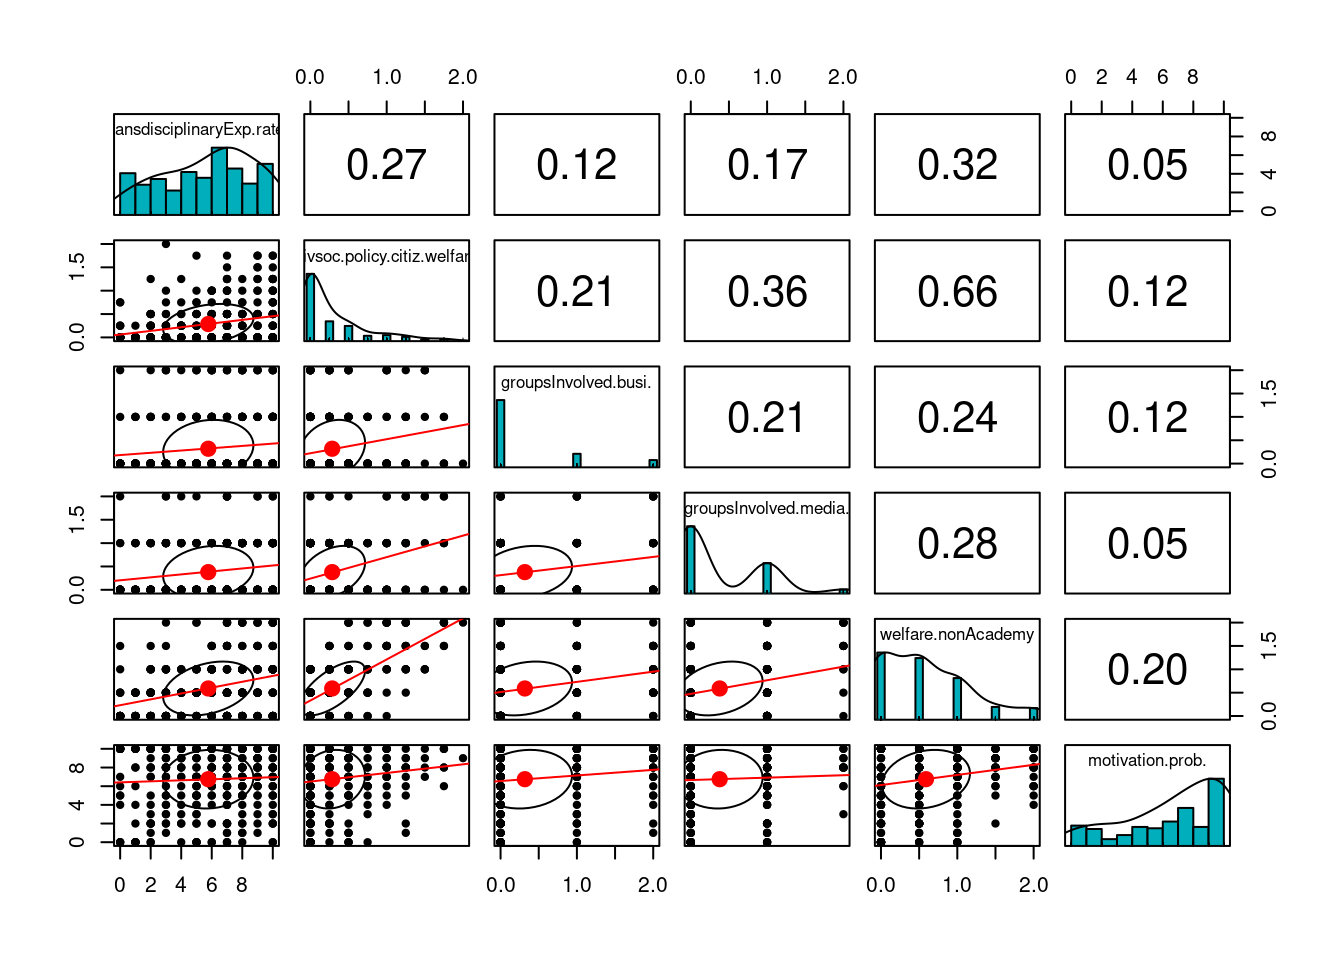
\includegraphics{model_description_files/figure-latex/unnamed-chunk-8-1.pdf}

\hypertarget{confirmatory-factory-analysis-theory-driven-model}{%
\subsubsection{Confirmatory Factory Analysis (Theory driven
model)}\label{confirmatory-factory-analysis-theory-driven-model}}

\begin{verbatim}
## lavaan 0.6-11 ended normally after 247 iterations
## 
##   Estimator                                         ML
##   Optimization method                           NLMINB
##   Number of model parameters                       126
##                                                       
##   Number of observations                           361
##                                                       
## Model Test User Model:
##                                                       
##   Test statistic                              3688.183
##   Degrees of freedom                               909
##   P-value (Chi-square)                           0.000
## 
## Model Test Baseline Model:
## 
##   Test statistic                              9363.946
##   Degrees of freedom                               990
##   P-value                                        0.000
## 
## User Model versus Baseline Model:
## 
##   Comparative Fit Index (CFI)                    0.668
##   Tucker-Lewis Index (TLI)                       0.639
## 
## Loglikelihood and Information Criteria:
## 
##   Loglikelihood user model (H0)             -21230.573
##   Loglikelihood unrestricted model (H1)     -19386.481
##                                                       
##   Akaike (AIC)                               42713.145
##   Bayesian (BIC)                             43203.144
##   Sample-size adjusted Bayesian (BIC)        42803.405
## 
## Root Mean Square Error of Approximation:
## 
##   RMSEA                                          0.092
##   90 Percent confidence interval - lower         0.089
##   90 Percent confidence interval - upper         0.095
##   P-value RMSEA <= 0.05                          0.000
## 
## Standardized Root Mean Square Residual:
## 
##   SRMR                                           0.086
## 
## Parameter Estimates:
## 
##   Standard errors                             Standard
##   Information                                 Expected
##   Information saturated (h1) model          Structured
## 
## Latent Variables:
##                               Estimate  Std.Err  z-value  P(>|z|)   Std.lv
##   fam =~                                                                  
##     fmlrWthSI.rsp.               1.000                               2.155
##     trnsdscplnrE..               0.772    0.096    8.024    0.000    1.663
##   ia_human_condition =~                                                   
##     motivatn.wlfr.               1.000                               2.567
##     benftFrNnAcdmy               0.263    0.017   15.427    0.000    0.674
##     implsFrNnAcd..               0.058    0.010    6.049    0.000    0.148
##     trgtGrpsGls.m.               0.149    0.011   14.051    0.000    0.382
##     implsFrNnAcd..               0.054    0.010    5.240    0.000    0.138
##     implsFrNnAcd..               0.002    0.008    0.305    0.760    0.006
##   ia_non_academic =~                                                      
##     implsFrNnAcd..               1.000                                  NA
##     implsFrNnAcd..               0.371    0.200    1.853    0.064       NA
##   transdisciplinary_social =~                                             
##     grpsInvlvd.ct.               1.000                               0.432
##     grpsInvlvd.cv.               0.680    0.067   10.125    0.000    0.294
##     grpsInvlvd.wl.               0.844    0.082   10.308    0.000    0.365
##     ntrOfInvlvmn..               0.733    0.076    9.691    0.000    0.316
##     ntrOfInvlvmn..               0.415    0.054    7.682    0.000    0.179
##     ntrOfInvlvmn..               0.768    0.079    9.750    0.000    0.332
##     trgtGrpsGls.s.               0.602    0.054   11.179    0.000    0.260
##     trgtGrpsGls.s.               0.508    0.047   10.913    0.000    0.219
##     trgtGrpsGls.m.               0.714    0.060   11.991    0.000    0.308
##     trgtGrpsGls.d.               0.637    0.063   10.184    0.000    0.275
##   outcome_public =~                                                       
##     impctTrgtGrp..               1.000                               1.878
##     impctTrgtGrp..               1.032    0.093   11.089    0.000    1.938
##     impctTrgtGrp..               0.977    0.098   10.014    0.000    1.835
##     impctTrgtGrp..               0.711    0.074    9.615    0.000    1.335
##     kindOfChng.pb.               0.153    0.023    6.738    0.000    0.288
##     kndOfChng.scg.               0.221    0.024    9.317    0.000    0.414
##     kndOfChng.wlf.               0.221    0.024    9.120    0.000    0.416
##     kndOfChng.cvs.               0.166    0.020    8.312    0.000    0.312
##   outcome_statement =~                                                    
##     Impctsttmnts..               1.000                               2.319
##     Impctsttmnts..               0.843    0.059   14.297    0.000    1.954
##     Impctsttmnts..               1.105    0.082   13.448    0.000    2.563
##     Impctsttmnts..               0.774    0.056   13.699    0.000    1.795
##     Impctsttmnts..               0.939    0.085   11.094    0.000    2.179
##     Impctsttmnts..               0.660    0.089    7.418    0.000    1.532
##   scale =~                                                                
##     sclbltyRtng.p.               1.000                               2.917
##     sclbltyRtng.t.               0.973    0.067   14.444    0.000    2.838
##     sclbltyRtng.d.               0.877    0.058   15.067    0.000    2.557
##   policy =~                                                               
##     grpsInvlvd.pl.               1.000                               0.455
##     impctTrgtGrp..               5.984    0.394   15.185    0.000    2.725
##     kndOfChng.plc.               1.460    0.113   12.894    0.000    0.665
##     ntrOfInvlvmn..               0.786    0.096    8.195    0.000    0.358
##     adptBPH.SQ001.               0.280    0.034    8.118    0.000    0.127
##   busi =~                                                                 
##     grpsInvlvd.bs.               1.000                               0.336
##     impctTrgtGrp..               7.811    0.792    9.858    0.000    2.628
##     kindOfChng.bs.               1.618    0.164    9.852    0.000    0.544
##   Std.all
##          
##     0.717
##     0.545
##          
##     0.753
##     0.861
##     0.338
##     0.766
##     0.294
##     0.017
##          
##        NA
##        NA
##          
##     0.668
##     0.589
##     0.601
##     0.561
##     0.438
##     0.565
##     0.658
##     0.640
##     0.713
##     0.593
##          
##     0.603
##     0.742
##     0.644
##     0.610
##     0.398
##     0.586
##     0.570
##     0.508
##          
##     0.735
##     0.768
##     0.724
##     0.737
##     0.602
##     0.407
##          
##     0.748
##     0.787
##     0.823
##          
##     0.721
##     0.884
##     0.724
##     0.459
##     0.454
##          
##     0.550
##     0.930
##     0.718
## 
## Covariances:
##                               Estimate  Std.Err  z-value  P(>|z|)   Std.lv
##   fam ~~                                                                  
##     ia_human_cndtn               3.086    0.474    6.503    0.000    0.558
##     ia_non_academc               0.076    0.039    1.958    0.050    0.518
##     trnsdscplnry_s               0.634    0.088    7.247    0.000    0.682
##     outcome_public               2.984    0.414    7.208    0.000    0.737
##     outcome_sttmnt               3.828    0.476    8.041    0.000    0.766
##     scale                        4.084    0.566    7.210    0.000    0.650
##     policy                       0.545    0.085    6.443    0.000    0.556
##     busi                         0.260    0.060    4.331    0.000    0.358
##   ia_human_condition ~~                                                   
##     ia_non_academc               0.070    0.039    1.799    0.072    0.398
##     trnsdscplnry_s               0.728    0.095    7.662    0.000    0.657
##     outcome_public               3.339    0.447    7.465    0.000    0.693
##     outcome_sttmnt               3.542    0.473    7.494    0.000    0.595
##     scale                        4.601    0.604    7.620    0.000    0.614
##     policy                       0.591    0.088    6.703    0.000    0.505
##     busi                         0.265    0.061    4.377    0.000    0.307
##   ia_non_academic ~~                                                      
##     trnsdscplnry_s               0.001    0.006    0.083    0.934    0.018
##     outcome_public               0.038    0.029    1.328    0.184    0.299
##     outcome_sttmnt               0.107    0.036    3.004    0.003    0.678
##     scale                        0.124    0.045    2.756    0.006    0.625
##     policy                       0.032    0.007    4.383    0.000    1.022
##     busi                         0.030    0.006    5.053    0.000    1.314
##   transdisciplinary_social ~~                                             
##     outcome_public               0.701    0.089    7.851    0.000    0.864
##     outcome_sttmnt               0.836    0.098    8.539    0.000    0.835
##     scale                        0.766    0.104    7.328    0.000    0.608
##     policy                       0.119    0.016    7.251    0.000    0.604
##     busi                         0.032    0.010    3.318    0.001    0.218
##   outcome_public ~~                                                       
##     outcome_sttmnt               3.630    0.451    8.053    0.000    0.833
##     scale                        4.135    0.534    7.738    0.000    0.755
##     policy                       0.565    0.078    7.219    0.000    0.660
##     busi                         0.177    0.045    3.932    0.000    0.279
##   outcome_statement ~~                                                    
##     scale                        5.214    0.605    8.612    0.000    0.771
##     policy                       0.774    0.093    8.287    0.000    0.733
##     busi                         0.258    0.056    4.621    0.000    0.331
##   scale ~~                                                                
##     policy                       0.935    0.115    8.114    0.000    0.704
##     busi                         0.448    0.079    5.657    0.000    0.456
##   policy ~~                                                               
##     busi                         0.047    0.011    4.362    0.000    0.306
##   Std.all
##          
##     0.558
##     0.518
##     0.682
##     0.737
##     0.766
##     0.650
##     0.556
##     0.358
##          
##     0.398
##     0.657
##     0.693
##     0.595
##     0.614
##     0.505
##     0.307
##          
##     0.018
##     0.299
##     0.678
##     0.625
##     1.022
##     1.314
##          
##     0.864
##     0.835
##     0.608
##     0.604
##     0.218
##          
##     0.833
##     0.755
##     0.660
##     0.279
##          
##     0.771
##     0.733
##     0.331
##          
##     0.704
##     0.456
##          
##     0.306
## 
## Variances:
##                    Estimate  Std.Err  z-value  P(>|z|)   Std.lv  Std.all
##    .fmlrWthSI.rsp.    4.393    0.614    7.149    0.000    4.393    0.486
##    .trnsdscplnrE..    6.554    0.578   11.341    0.000    6.554    0.703
##    .motivatn.wlfr.    5.032    0.472   10.670    0.000    5.032    0.433
##    .benftFrNnAcdmy    0.158    0.021    7.445    0.000    0.158    0.258
##    .implsFrNnAcd..    0.171    0.013   13.178    0.000    0.171    0.886
##    .trgtGrpsGls.m.    0.103    0.010   10.417    0.000    0.103    0.413
##    .implsFrNnAcd..    0.201    0.015   13.248    0.000    0.201    0.914
##    .implsFrNnAcd..    0.125    0.009   13.434    0.000    0.125    1.000
##    .implsFrNnAcd..    0.079    0.017    4.502    0.000    0.079    1.063
##    .implsFrNnAcd..    0.157    0.012   13.190    0.000    0.157    1.004
##    .grpsInvlvd.ct.    0.231    0.019   12.226    0.000    0.231    0.553
##    .grpsInvlvd.cv.    0.162    0.013   12.642    0.000    0.162    0.653
##    .grpsInvlvd.wl.    0.235    0.019   12.592    0.000    0.235    0.639
##    .ntrOfInvlvmn..    0.217    0.017   12.749    0.000    0.217    0.685
##    .ntrOfInvlvmn..    0.135    0.010   13.083    0.000    0.135    0.808
##    .ntrOfInvlvmn..    0.235    0.018   12.736    0.000    0.235    0.681
##    .trgtGrpsGls.s.    0.089    0.007   12.292    0.000    0.089    0.567
##    .trgtGrpsGls.s.    0.069    0.006   12.396    0.000    0.069    0.590
##    .trgtGrpsGls.m.    0.092    0.008   11.880    0.000    0.092    0.492
##    .trgtGrpsGls.d.    0.139    0.011   12.626    0.000    0.139    0.648
##    .impctTrgtGrp..    6.163    0.493   12.504    0.000    6.163    0.636
##    .impctTrgtGrp..    3.060    0.269   11.375    0.000    3.060    0.449
##    .impctTrgtGrp..    4.762    0.388   12.278    0.000    4.762    0.586
##    .impctTrgtGrp..    3.010    0.241   12.470    0.000    3.010    0.628
##    .kindOfChng.pb.    0.439    0.033   13.134    0.000    0.439    0.842
##    .kndOfChng.scg.    0.329    0.026   12.588    0.000    0.329    0.657
##    .kndOfChng.wlf.    0.359    0.028   12.656    0.000    0.359    0.675
##    .kndOfChng.cvs.    0.279    0.022   12.874    0.000    0.279    0.742
##    .Impctsttmnts..    4.565    0.390   11.715    0.000    4.565    0.459
##    .Impctsttmnts..    2.652    0.234   11.315    0.000    2.652    0.410
##    .Impctsttmnts..    5.945    0.503   11.826    0.000    5.945    0.475
##    .Impctsttmnts..    2.702    0.231   11.695    0.000    2.702    0.456
##    .Impctsttmnts..    8.340    0.661   12.619    0.000    8.340    0.637
##    .Impctsttmnts..   11.829    0.899   13.153    0.000   11.829    0.834
##    .sclbltyRtng.p.    6.691    0.611   10.952    0.000    6.691    0.440
##    .sclbltyRtng.t.    4.951    0.484   10.226    0.000    4.951    0.381
##    .sclbltyRtng.d.    3.105    0.336    9.249    0.000    3.105    0.322
##    .grpsInvlvd.pl.    0.192    0.017   11.394    0.000    0.192    0.480
##    .impctTrgtGrp..    2.072    0.304    6.826    0.000    2.072    0.218
##    .kndOfChng.plc.    0.402    0.035   11.360    0.000    0.402    0.476
##    .ntrOfInvlvmn..    0.481    0.037   12.957    0.000    0.481    0.790
##    .adptBPH.SQ001.    0.062    0.005   12.969    0.000    0.062    0.793
##    .grpsInvlvd.bs.    0.261    0.021   12.423    0.000    0.261    0.698
##    .impctTrgtGrp..    1.077    0.431    2.502    0.012    1.077    0.135
##    .kindOfChng.bs.    0.278    0.028    9.985    0.000    0.278    0.484
##     fam               4.643    0.785    5.915    0.000    1.000    1.000
##     ia_human_cndtn    6.591    0.831    7.933    0.000    1.000    1.000
##     ia_non_academc   -0.005    0.016   -0.285    0.775       NA       NA
##     trnsdscplnry_s    0.186    0.027    6.894    0.000    1.000    1.000
##     outcome_public    3.528    0.585    6.030    0.000    1.000    1.000
##     outcome_sttmnt    5.380    0.685    7.857    0.000    1.000    1.000
##     scale             8.506    1.076    7.909    0.000    1.000    1.000
##     policy            0.207    0.028    7.534    0.000    1.000    1.000
##     busi              0.113    0.022    5.260    0.000    1.000    1.000
\end{verbatim}

\textbf{Observations:}

\begin{itemize}
\tightlist
\item
  Goodness of fit, Chi-Squared p value is very small (0.000)
\item
  CFI and TFI are questionable but not too low (\textasciitilde0.65),
  normailly expected \textasciitilde0.9
\item
  RMSEA is surprisingly high (0.092) and stat. significant (0.000), the
  values I've seen so far were always \textasciitilde0.05 and rarely
  significant
\item
  SRMR is high (0.086), indication of a good fitting model.
\item
  P values of the loadings are almost too good other than a couple of
  variables (to be addressed)
\item
  Covariances are to be discussed
\item
  Variance estimates are to be discussed (e.g.~ia\_non:academic has very
  low variance -0.0005, what does it indicate)
\end{itemize}

\hypertarget{model-output}{%
\section{Model Output}\label{model-output}}

\hypertarget{correlation-between-the-self-assessment-si-rate-and-the-prediction}{%
\subsection{\texorpdfstring{Correlation between the \emph{self
assessment SI-Rate} and the
prediction}{Correlation between the self assessment SI-Rate and the prediction}}\label{correlation-between-the-self-assessment-si-rate-and-the-prediction}}

\begin{center}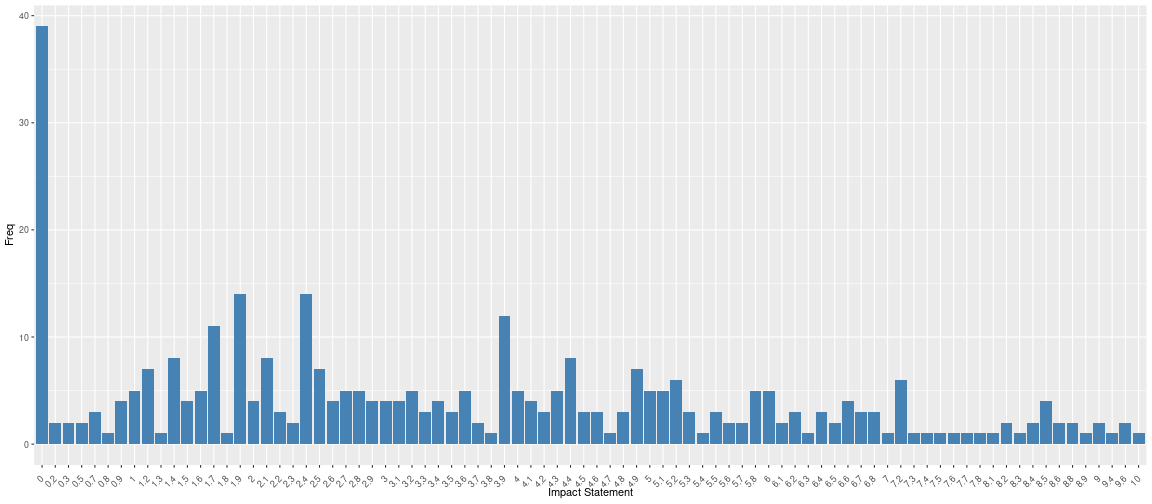
\includegraphics[width=720px]{model_description_files/figure-latex/unnamed-chunk-12-1} \end{center}

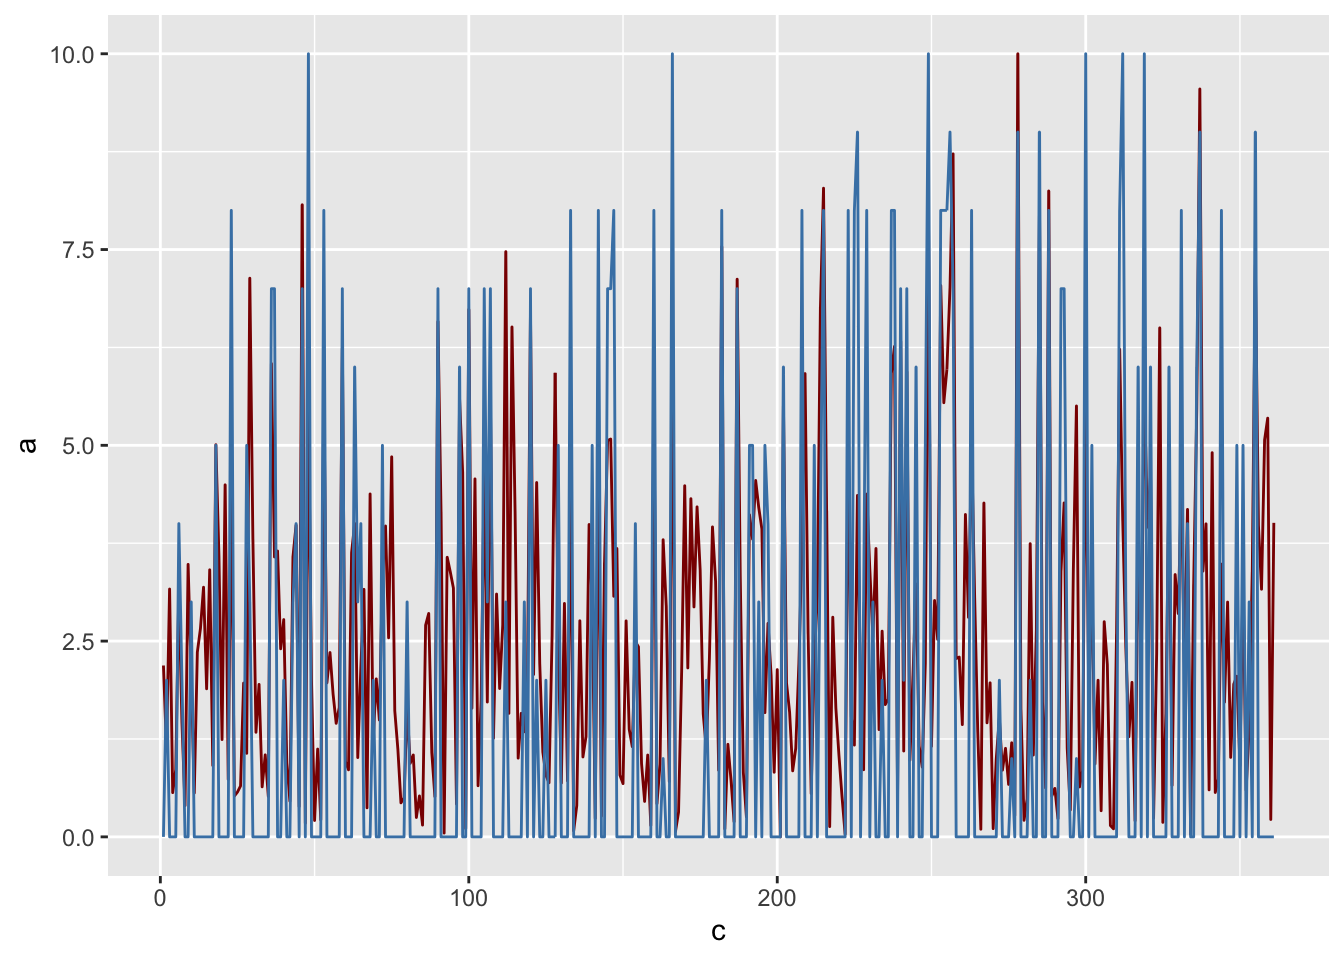
\includegraphics{model_description_files/figure-latex/unnamed-chunk-13-1.pdf}

\hypertarget{how-to-create-a-re-appliable-formulation}{%
\section{How to Create a (Re-)Appliable
Formulation}\label{how-to-create-a-re-appliable-formulation}}

\end{document}
